\documentclass[a4paper]{llncs}

\usepackage{amssymb}
\setcounter{tocdepth}{3}
\usepackage{graphicx}

\usepackage{url}
\urldef{\mailsa}\path|{pghilardi,ricardo}@inf.ufsc.br| \newcommand{\keywords}[1]{\par\addvspace\baselineskip
\noindent\keywordname\enspace\ignorespaces#1}

\begin{document}

\mainmatter  % start of an individual contribution

% first the title is needed
\title{SEA/Aspect: Dynamic Visualization and Composition of Concerns in Aspect-Oriented Modeling (AOM)}

% the name(s) of the author(s) follow(s) next  NB: Chinese authors should write their first names(s) in front of their surnames. This ensures that the
% names appear correctly in the running heads and the author index.
\author{Pedro Ghilardi, Ricardo Pereira e Silva}
%  (feature abused for this document to repeat the title also on left hand pages)

% the affiliations are given next; don't give your e-mail address unless you accept that it will be published
\institute{Federal University of Santa Catarina\\
Department of Informatic and Statistics\\
Florian�polis, Santa Catarina - Brasil\\
\mailsa\\
}

%  NB: a more complex sample for affiliations and the mapping to the corresponding authors can be found in the file "llncs.dem" (search for the string
% "\mainmatter" where a contribution starts).
% "llncs.dem" accompanies the document class "llncs.cls".

\maketitle

\bibliographystyle{splncs}

\begin{abstract}
The Aspect-Oriented Modeling (AOM) aims to raise the abstraction level from code
to models in the representation of aspect-oriented systems. This paper aims at the 
representation of aspect-oriented software using UML, through a lightweight profile, modeling the most important features 
of Aspect-Oriented Programming (AOP) and enabling alternating views of the
system dynamics. The developer may create different compositions of the core and 
the crosscutting models, visualizing only the core models, the
crosscutting models, or the core intertwined with the crosscutting models. The visualization of 
the aspect dynamic can be enabled or disabled dynamically, by updating the compound model, with no effort
demanded from the developer. The concerns are differentiated in the compound
model by different colors. The proposed solution is implemented as a tool, named
SEA/Aspect, that enables the automatic generation of sequence diagrams resulting from 
the intertwining of aspects, which also allows the selection of which aspects will be composed.
\end{abstract}

\keywords{Aspect-Oriented Modeling, UML, Model Composition, Model
Visualization, Model Weaving, Modeling Tool}

\section{Introduction}

A system consists of a set of requirements, where each requirement can be considered a customer{'}s concern. The core concerns captures the
core functionality and impact only a part of the system, while the crosscutting concerns captures functionality that impacts one or more
parts of the system. The AOP{'}s goal is the modularization of these concerns, so that they are kept in separate modules
that implement the core concerns of an application \cite{Laddad:2003:AAP:993468}.

The most elementary way to represent aspect-oriented programs is directly at the code level. One of the limitations of this approach is that the concerns
modularization makes it difficult to understand the execution flow, since the system dynamic is visualized only after the composition of concerns, or
with the aid of tools for visualizing the effect of the aspects in the system core. Another limitation of the direct implementation in code is that
with the low-level of abstraction, the developer may be overwhelmed with implementation details rather than on the interaction of the core and
crosscutting concerns. 

An aspect-oriented system demands the representation of the characteristics inherent to AOP and may have their understanding facilitated by
alternating the views of the application dynamic, visualizing the crosscutting concerns composed with the core concerns. As we
are working in the modeling of aspect-oriented applicatons, the model of a crosscutting concern will be referred as a crosscutting model and the model
of a core concern as a core model. The Unified Modeling Language (UML), the standard language used to model object-oriented systems \cite{uml:05},
could be used for aspect-oriented systems, but it have elements that cannot be represented with the standard meta-model. To overcome this limitation,
the language could be extended by two ways: via a lightweight extension through a profile, or an extension through the modification of the language
meta-model.

Some approaches have been proposed for the modeling of aspect-oriented systems using UML. A group of proposals extends the language meta-model
\cite{Kienzle:2009:AMM:1509239.1509252} \cite{theme:04} \cite{Klein:2007:WMA:1805812.1805819} \cite{Jacobson:2004:ASD:1062430}
\cite{Zhang:2012:WSA:2162049.2162080}, introducing non-standard language constructs to represent the structure and behavior of aspect-oriented
applications. Another set of proposals extends the UML through a lightweight profile \cite{Evermann:2007:MSP:1229375.1229379}
\cite{Cottenier06themotorola} \cite{stein:02}, which can be used in CASE tools that support importing profiles. Our approach specifies aspect-oriented
software through a lightweight profile, using some stereotypes from the Evermann{'}s \cite{Evermann:2007:MSP:1229375.1229379} profile and proposing
others to represent the behavior of the core and crosscutting concerns. The constructions are based in the AspectJ language \cite{AspectJ11}, which is
the standard language for AOP with Java. The proposed approach allows the capture of multiple join points with wildcards in the pointcut specification
and the modeling of the most important characteristics of AOP. The constructions specified by the lightweight profile allows the automatic composition of
core and crosscutting models, enabling alternating views of the system dynamics (with and without the explicitation of the aspects) and, thus,
facilitating the model understanding and maintenance. The SEA/Aspect, implemented in the SEA environment \cite{silva:00} as a tool, allows the dynamic
enabling of aspects, visualizing only the behavior of the core models, the crosscutting models, or the composition of one or more crosscutting models
with a core model automatically. The developer differentiates the behavior of each concern by different colors in the compound model.

This article is organized as follows: section II presents the related work. Section III presents the proposal for specification of aspect-oriented
software. The section IV deals with the aspects composition and the visualization toggling tool. Section V presents a case study using the proposed
tool. The limitations are in the section VI and the conclusions in the section VII.
 
\section{Related Work}

Some studies have been done in the modeling of aspect-oriented applications. Some approaches extends the UML using a profile, while others create a
customized meta-model. Most approaches represents the structure of aspect-oriented applications, but some also represent its behavior. The automatic 
composition of models is a desired feature, because it allows the toggle of views and automates part of the modeling. According to Fuentes
\cite{fuentes-profile:1755547}, although each form of extension has its advantages and disadvantages, in most cases, the extension through a profile 
is better than extending the meta-model, because the meta-model extensions cannot be used in CASE available tools.

The proposals that are presented next extends the UML through profiles. Evermann{'}s \cite{Evermann:2007:MSP:1229375.1229379} proposes a profile to
model the structure of aspect-oriented applications. Some stereotypes proposed by him are used in this work, as the definition of aspects and
crosscutting concerns. One of the main contributions of Evermann{'}s work is the representation of aspect-oriented applications only within UML terms,
without textual specifications. But using only UML terms, it is not possible to capture multiple join points with wildcards in the pointcut
specification. Our approach represents pointcuts with states and transitions from the UML state machine diagram, which allows the specification of
wildcards. The Motorola WEAVR \cite{Cottenier06themotorola} uses the UML state machine diagram to represent pointcuts and advices, extending its
semantics through a lightweight profile. The aspects are modeled using state machines focused in transitions, instead the traditional state machines
that are focused in the states. However, the modeling is in a low-level of abstraction with constructions close to the target language code. Our
approach also differentiates from Cottenier{'}s in the modeling of advices. While it models advices with the UML state machine diagram, we use the UML
sequence diagram to represent the advices as a set of messages. In our approach, the connection between pointcuts and advices is obtained with the use
of state invariants, which are added in the sequence diagrams. When the system mets a pointcut, it enters in a state, this state is referred as a
state invariant in the sequence diagram and triggers the execution of the advice. The Stein{'}s approach \cite{stein:02}
\cite{Stein:2006:EDC:1119655.1119661} \cite{Hanenberg:2007:ADA:1218563.1218570} allows the specification of aspect-oriented applications through a
profile. However, the main objective of the approach is the automatic generation of code from aspect-oriented models, while our approach performs
weaving of core and crosscutting models in the modeling level.

The extension through meta-modeling is a characteristic of the approaches presented from now. A multi-view modeling is proposed by Kienzle
\cite{Kienzle:2009:AMM:1509239.1509252}, extending the UML meta-model. The Reusable Aspect Models (RAM) models the structure of applications using the
class diagram, and the behavior using the sequence and state machine diagrams. Introductions are modeled with class diagrams. Pointcuts and advices
are represented with sequence and state machine diagrams. The modeling does not represents the connection between pointcuts and sequence diagrams. In
this paper, the pointcuts are defined in state machines and the connection between pointcuts and sequence diagrams is realized using state invariants,
which is not specified in the RAM approach. The main contributions of RAM is that it allows a complete representation of an aspect-oriented
application in the modeling phase, using class, sequence and state machine diagrams. Another important contribution is the extensive consistency
checks in the weaving and on compound models. Klein{'}s approach \cite{Klein:2007:WMA:1805812.1805819} uses extended sequence diagrams to model the
system behavior and allows the composition of multiple aspects in the same joinpoint. However, the approach of Klein does not allow the representation
of pointcuts with wildcards. Jacobson{'}s approach \cite{Jacobson:2004:ASD:1062430} represents aspects in terms of use cases. A construction named
use-case slice (with the stereotype \textit{use case slice}) groups all the models of a concern, which includes introductions and collaborations. Our
approach uses the Hotel Management System presented in Jacobson{'} work to assess the specification of aspect-oriented software. One of the
limitations of the approach is the need to compose the aspect models manually, which increases the time spent in the modeling, while our approach
allows the automatic composition of models. Theme/UML \cite{theme:04} supports the modeling of core and crosscutting concerns, automates the
composition of models and represents the most important features of AOP. Theme/UML modifies the UML meta-model and is dependent on the version 1.3 of
the language. Carton{'}s proposal \cite{Carton:2009:MT:1692821.1692829} aims to overcome this limitation, creating a marking profile to represent
Theme/UML accordingly to the UML standards. However, the model composition is still limited to the constructs available on the version 1.3 of the UML.
High-Level Aspects (HiLA) \cite{HiLA} uses state machines to model aspect-oriented applications. Pointcuts and advices are modeled using states and
transitions. In comparison with graph-transformation approaches, that also uses state machines to describe aspects, the models created with HiLA are
more easier to construct and understand. A tool that performs the composition (weaving) of aspects is proposed in a recent contribution
\cite{Zhang:2012:WSA:2162049.2162080}, which automates part of the modeling process. However, HiLA changes the UML meta-model to represent aspect-oriented 
applications, and cannot be used in available CASE tools.

\section{Specification of Aspect-Oriented Software}

Figure \ref{fig:full_profile} shows the UML profile to represent the structure and behavior of aspect-oriented applications. The profile may be used
in CASE tools that support importing profiles through the XML Metadata Interchange (XMI) \cite{xmi:11}. Relative to the structural modeling, this
paper uses some definitions from the Evermann{'}s profile \cite{Evermann:2007:MSP:1229375.1229379}, which allows the representation of the AOP{'}s
structural characteristics. The definitions used from Evermann{'}s profile are the \textit{CrosscuttingConcern} and the \textit{Aspect} stereotypes,
that are colored in beige in the profile diagram. A stereotype extends an element from the UML meta-model improving its semantics.
In this paper, a meta-model element being extended will be represented inside parentheses. The \textit{CrosscuttingConcern} stereotype extends
(\textit{Package}) and contains a set of aspects and classes. It represents a concern that impacts one or more parts of the system. The
\textit{Aspect} stereotype extends (\textit{Class}), contains inter-type declarations and some configuration properties as:
type of aspect instantiation, associated pointcut and a flag to indicate if this aspect is privileged. Inter-type declarations allows injection of
members (method, attribute) on a class, change of inheritance hierarchy and interfaces implementation. To represent inter-type declarations, a
stereotype denominated \textit{ClassExtension} was created. This stereotype extends (\textit{Class}) and is related to another stereotype named
\textit{Introduction}. The \textit{Introduction} stereotype is used to mark which member is being inserted on a given class, or which inheritance
relationship is being added, or which interface is being implemented. The stereotype \textit{Introduction} extends the meta-model elements 
(\textit{Attribute}), (\textit{Operation}), (\textit{Generalization}) and (\textit{Realization}). Due to space limitations, we will not go into details 
regarding the structural modeling, which can be fully implemented using the proposed stereotypes. 

\begin{figure}[!h]
	\centering
	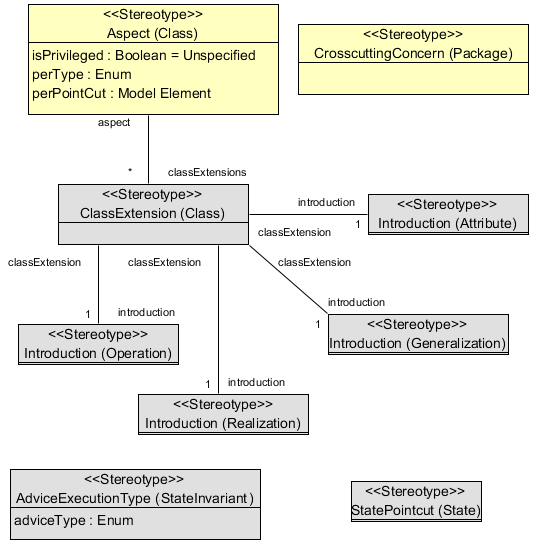
\includegraphics[scale=0.5]{img/full_profile.png}
	\caption{UML Profile to model Aspect-Oriented
	Applications.}\label{fig:full_profile}
\end{figure}

Besides inter-type declarations and aspect configurations, an aspect contains pointcuts and advices. Evermann{'}s profile
\cite{Evermann:2007:MSP:1229375.1229379} represents pointcuts within the aspect definition, but without the possibility of capturing multiple join
points in the pointcut specification. Our approach represents pointcuts with the UML state machine diagram. Each transition represents the capture of
one or more join points, with the possibility of using wildcards. If the capture of all the join points is satisfied, that is, if the conditions for
triggering a transition are satisfied, it is considered that the system has met a certain pointcut. The stereotype \textit{StatePointcut} extends
(\textit{State}) and represents a pointcut. The composition of pointcuts is achieved by composing different state machines. The stereotype that
represents pointcuts can be seen in the bottom right of figure \ref{fig:full_profile}. Figure \ref{fig:pointcut_definition_1} shows the definition of
pointcuts using the proposed approach. The pointcut \textit{AnyCall} captures calls (\textit{call} pointcut) to any method of any class, using a
wildcard to match any return type, any class and any method name with any number of parameters. The pointcut \textit{RoomTarget} captures the
occurences of a call when the target object (\textit{target} pointcut) is of the type \textit{Room}. Each pointcut is represented as a state in the
state machine diagram. The pointcut signature is specified in the transition, which allows the use of wildcards to capture multiple joinpoints. When
the pointcut state is reached, it means that the system has captured the execution points specified by the pointcut signature in the transition label.

\begin{figure}[h]
	\centering
	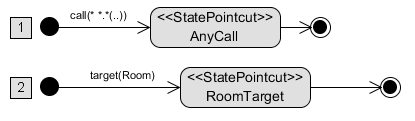
\includegraphics[scale=0.5]{img/pointcut_definition_1.png}
	\caption{The definition of two
	pointcuts.}\label{fig:pointcut_definition_1}
\end{figure}

The AspectJ language allows the composition of pointcuts with the logical operators \textit{and}, \textit{or} and \textit{not}. The proposed approach
performs the automatic composition of pointcuts using state machine digrams. Figure \ref{fig:pointcut_definition_and} shows the composition of the
pointcuts \textit{AnyCall} and \textit{RoomTarget} using the \textit{and} operator. The compound state machine contains a state with a
\textit{concurrent region}, containing sub-states that execute concurrently: \textit{AnyCall} and \textit{RoomTarget}. The synchronization occurs with
the \textit{fork} and \textit{join} nodes, which means that the final state (\textit{AnyCall AND RoomTarget}) only will be reached if both states
(\textit{AnyCall} and \textit{RoomTarget}) are reached. This is the semantic of the \textit{and} operator in the AspectJ language. Figure
\ref{fig:pointcut_definition_or} shows the composition of the pointcuts using the \textit{or} operator. Here the semantics is a bit different, because
the system will reach the final state (\textit{AnyCall OR RoomTarget}) when any of the pointcuts are reached. This is represented in the compound
state machine, that shows direct transitions from both states to the final state.

\begin{figure}[h]
	\centering
	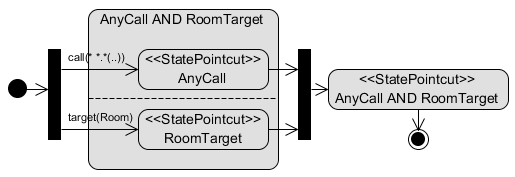
\includegraphics[scale=0.5]{img/pointcut_definition_and.png}
	\caption{The composition of two pointcuts
	with the AND operator.}\label{fig:pointcut_definition_and}
\end{figure}

\begin{figure}[h]
	\centering
	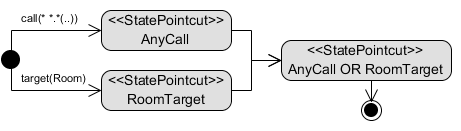
\includegraphics[scale=0.5]{img/pointcut_definition_or.png}
	\caption{The composition of two pointcuts
	with the OR operator.}\label{fig:pointcut_definition_or}
\end{figure}

A pointcut only captures the execution points of a system. The behavior to be injected in these points is represented by the advice, that is directly
associated with a pointcut. Sequence diagrams are used to represent the behavior of the core concerns (core model) and the crosscutting concerns
(crosscutting models). An aspect may have one or more advices and each one is represented by a crosscutting model. The behavior of an advice executes
when its associated pointcuts are satisfied, i.e, all joint points are captured. As we model pointcuts with the state machine diagram and advices with
the sequence diagram, the connection of the advices with pointcuts should be achieved using syntatic elements of these diagrams. We implement this
connection using state invariants. A state invariant is an interaction fragment associated with a lifeline on the sequence diagram, representing a run-time 
constraint on the participants of the interaction. We use the reachability of a state as the constraint to trigger the advice execution.

The definition of a crosscutting model (as a sequence diagram) begins adding the aspect as the first lifeline of the diagram. A state invariant, which
represents the satisfaction of a pointcut, is associated to the aspect lifeline. This means that the sequence of messages occurs only when the system
reaches the state represented by the state invariant. The messages may be executed before, after or around the triggering of a pointcut. The execution
time is configured using the \textit{AdviceExecutionType} stereotype. This stereotype extends (\textit{StateInvariant}) and can be seen in the bottom
left of figure \ref{fig:full_profile}. The \textit{AdviceExecutionType} has the tagged value \textit{adviceType} of enumeration type. The valid
types of the enumeration are: before, after or around.

The connection between advice and pointcuts can be better understood in the example of figure \ref{fig:behavioral_profile_example}. This figure
shows the pointcut previously specified to capture any method call on any class with any numbers of parameters (\textit{AnyCall}). The log aspect
defines a crosscutting model that logs a message using a \textit{Logger}. The crosscutting model is described as a sequence of messages in a sequence
diagram. This diagram contains a state invariant that refers to the \textit{AnyCall} pointcut. A state invariant must have the advice execution type
stereotype and the advice type tagged value to specify when the advice behavior will be executed. In this example, the advice behavior
will be executed \textit{after} the execution points captured by the \textit{AnyCall} pointcut. The message \textit{log()} will be executed only when
the state \textit{AnyCall} is achieved.

\begin{figure}[h]
	\centering
	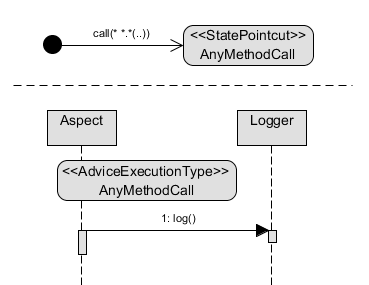
\includegraphics[scale=0.5]{img/behavioral_profile_example.png}
	\caption{The connection between
	pointcuts and advices using state
	invariants.}\label{fig:behavioral_profile_example}
\end{figure}

\section{Visualization Toggling and Composition of Aspects}

The profile is added to the SEA environment \cite{silva:00}, which supports UML diagramming. The SEA/Aspect is a tool which allows the selection of
which crosscutting models will be intertwined together with the core models of the system. One can automatically visualize only the core models, the
crosscutting models, or core intertwined with crosscutting models. Aspects can be enabled or disabled dynamically, by updating the compound model,
with no effort demanded from  the developer. This automatic updating allows the toggling of views, visualizing different models compositions. The
SEA/Aspect has two different phases to output a compound model: \textbf{selection} and \textbf{composition}, which are described in the next sections.

\subsection{Selection}
  
The developer selects which core and crosscutting models to compose and assign a different color to each model. These colors differentiate the
elements of each model in the compound model. One or more aspects can be composed at the same time. The selected aspects are the input to the second
phase, that is the composition of the core and crosscutting models.

\subsection{Composition}

The composition is made between a core model and one or more crosscutting models, and provides, as a result, a compound model with the structure or
behavior of the crosscutting models injected into the core models. In the compound model, the croscutting behavior differs from the core behavior by
different colors, as illustrated in figure \ref{fig:case_study_compound_2}. The composition algorithm has the \textbf{match} and \textbf{merge}
activities. The first activity locates the captured concepts in the core model and the last weaves the structure or behavior of the crosscutting
models in the core model, giving as result a compound model. SEA/Aspect allows the automatic composition of class and sequence diagrams. Due to space
reasons, the composition of class diagrams will not be explained.

The \textbf{composition of sequence diagrams} uses wildcard matching and has the following steps:
  
	\begin{itemize}
	  \item \textbf{Match:} With the core and crosscutting models selected by the developer, the composert finds the 
	  execution points of the core model that are impacted by the crosscutting models. This information is obtained from the pointcuts defined in the 
	  crosscutting models. The algorithm is separated in three steps:
	  \begin{enumerate}
	    \item \textbf{Find the pointcut:} To obtain the pointcut from the
	    crosscutting sequence diagram (crosscutting model), the algorithm looks for the state invariants 
	    stereotyped as \textit{AdviceExecutionType}. The state invariant maps to
	    the state that defines the pointcut.
	    \item \textbf{Separate the pointcut:} The composer uses a regular
	    expression to separate a pointcut in four parts: \textbf{pointcut type}, \textbf{return type pattern},
	  \textbf{identification pattern} and \textbf{exception pattern}. 
	  The pointcut type is mandatory and is one of the types supported by the
	  AspectJ language, which includes \textit{execution}, \textit{call}, 
	  \textit{this} and others. The return type pattern is optional and specifies the return
	  type of the pointcut. The identification pattern is mandatory and contains
	  the signature to be matched in the core model. Finally, the exception pattern
	  is optional too, and is used to capture execution points that throws
	  exceptions of a given type
	    \item \textbf{Match the execution points:} The composer uses regular
	    expressions to match which execution points are impacted by the pointcuts defined in the crosscutting 
	  models. This match support pointcuts specified with wildcards, that is an
	  important feature of aspect-oriented languages. It starts using the
	  identification pattern to find context information about the impacted 
	  concepts, like package and class context of a given method, for example. 
	  When all concepts inside a given context are captured, the algorithm uses
	  another regular expression to match the names of the captured concepts. 
	  For instance, when matching a method, the algorithm check return type,
	  parameters (name, type and number of parameters) and the method signature. 
	  Finally, the composer check for exception throws, if any. As output, the
	  concepts (classes and methods) impacted by the crosscutting models are
	  stored to be used in the merge activity.
	  \end{enumerate}  
	  
	  \item \textbf{Merge:} Merge concepts of the crosscutting models with
	  the impacted core model concepts. The merge receives as input the impacted
	  core model concepts that should be merged with croscutting ones. The merge
	  purpose is to inject a set of messages, lifelines, combined fragments and
	  other sequence diagram concepts in the core sequence diagram (core model),
	  adding new behavior defined in the crosscutting sequence diagrams
	  (crosscutting models). To achieve this, the algorithm is separated in
	  two steps:
		  \begin{enumerate}
		    \item \textbf{Find the advice execution type:} Retrieve the advice execution type from the
		    state invariant defined by the crosscutting model. The supported advice
		    types are: \textit{before}, \textit{around} and \textit{after} and are defined in 
		    the tagged value advice type. The advice type gives the
		    information of when the messages should be injected in the core sequence diagram.
		  	\item \textbf{Inject the messages:} At this time, the algorithm knows the
		  	impacted concepts, the messages to inject from the crosscutting model 
		  	and when the messages should be inserted. The next
		  	step is the messages injection and reordering, because the injection of a
		  	message triggers a reordering event in the sequence diagram. With all
		  	the messages injected and ordered, the composer paints each message name
		  	with the correspondent crosscutting model color, to differentiate which
		  	message comes from which aspect. The merge produces as output a compound
		  	sequence diagram with the crosscutting concepts composed in the core
		  	sequence diagram.
		  \end{enumerate}
	  \end{itemize}  

\section{Case Study}\label{sec:case_study}

This section presents a case study to assess the applicability of the proposed approach in the modeling of an application. The case study is based in
the Hotel Management System extracted from Jacobson{'}s book \cite{Jacobson:2004:ASD:1062430}. This example allows the modeling of important
aspect-oriented funcionalities and is consolidated in the literature. The use cases represented in this case study are the reservation of rooms,
handling of a waiting list of customers and the logging of messages. As we are not going into details about the modeling of the structure of
aspect-oriented software, the structural diagrams of the case study will not be show in this section, although they can be represented using the
stereotypes of the UML profile.

Sequence diagrams are used to represent the behavior of the core and crosscutting concerns, using the profile and the process proposed by this
approach. The modeling of concerns using behavioral diagrams gives subsidies to achieve the toogling of views, that allows better understanding of
aspect-oriented applications, visualizing the effect of the aspects in the system. We start with the sequence diagram of the reserve room concern,
that is show in figure \ref{fig:case_study_behavioral_reserve_room}. In a room reservatiom, if the room isn't available, an exception is raised in the
method \textit{updateAvailability()}, otherwise, the reservation is done and the customer receives a confirmation code.

  \begin{figure}[!b]
	\centering
	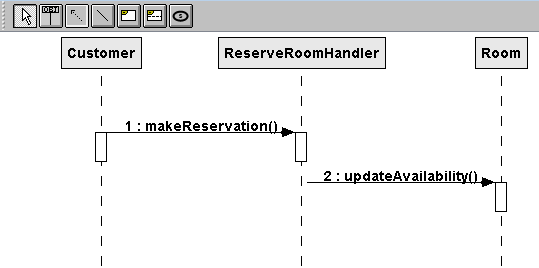
\includegraphics[scale=0.5]{img/case_study_behavioral_reserve_room.png}
	\caption{Advice behavior of the core concern to reserve a room.}\label{fig:case_study_behavioral_reserve_room}
  \end{figure}
  
The other concerns to be modeled are the crosscutting concerns that contains pointcuts and advices. The log concern needs to account the number of
requests to a room. To achieve this, we must define a pointcut that captures the calls to the \textit{Room} class. This pointcut is modeled using the
state machine diagram and is show in figure \ref{fig:case_study_behavioral_pointcut_log}. With the pointcut defined, we create the sequence diagram to
the log concern. The diagram is show in figure \ref{fig:case_study_behavioral_log} and contains as the first lifeline the \textit{LogAspect}.
Accordingly to the proposed approach, an aspect in the sequence diagram must have a state invariant associated, which is the trigger to execute the
sequence of messages. In this case, the state invariant \textit{RoomCall} is associated with the \textit{LogAspect} and points to a pointcut
previously defined in the state machine diagram. The semantics here is that the sequence of messages will execute only when the pointcut is satisfied.
The message to be executed when the pointcut is satisfied is a call to the method \textit{log()} of the \textit{Logger} class. It is important to be
aware of the advice type, that is defined as a tagged value in the state invariant. The tagged value is not being show in the sequence diagram to
not clutter the diagram. The proposed approach supports three types of advice types: before, after or around. In this case, the advice type is after,
which means that the log behavior will execute after any method call to the \textit{Room} class. The sequence diagram contains a combined fragment of 
type optional, that defines that the log only will be performed if the application is not frozen. An application is not frozen when it is running in the development environment.

  \begin{figure}[tb]
	\centering
	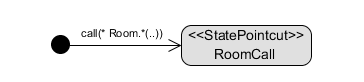
\includegraphics[scale=0.5]{img/case_study_behavioral_pointcut_log.png}
	\caption{Pointcut of the crosscutting concern to log messsages.}\label{fig:case_study_behavioral_pointcut_log}
  \end{figure}
  
  \begin{figure}[tb]
	\centering
	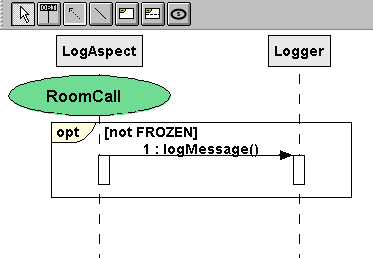
\includegraphics[scale=0.5]{img/case_study_behavioral_log.png}
	\caption{Advice behavior of the crosscutting concern to log messages.}\label{fig:case_study_behavioral_log}
  \end{figure}

The last concern to be modeled is the waiting list, that adds the customer to a waiting list when a room isn't available. To achieve this, we need a
pointcut that captures when a customer try to reserve a room without success, because it is unavailable. Figure
\ref{fig:case_study_behavioral_pointcut_waiting_list} shows a pointcut that captures calls to the method \textit{updateAvailability()} of the
\textit{Room} class, raising the \textit{NoRoomsAvailable} exception. Besides the pointcut definition, we need to define the behavior of how a
customer is added to the waiting list. This behavior is modeled in the sequence diagram of figure \ref{fig:case_study_behavioral_waiting_list}. The
diagram has the \textit{WaitingListAspect} as the first lifeline and has a sequence of messages to be executed when the system raises an exception
that no rooms are available. These messages will be executed after the exception raising, because the advice type of the state invariant is after.
Again, the tagged value is not being show in the sequence diagram to not clutter the diagram.

  \begin{figure}[tb]
	\centering
	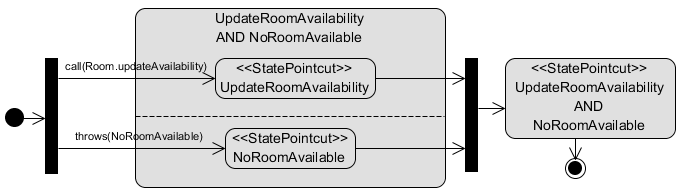
\includegraphics[scale=0.5]{img/case_study_behavioral_pointcut_waiting_list.png}
	\caption{Pointcut of the crosscutting concern to handle a waiting list.}\label{fig:case_study_behavioral_pointcut_waiting_list}
  \end{figure}
  
  \begin{figure}
	\centering
	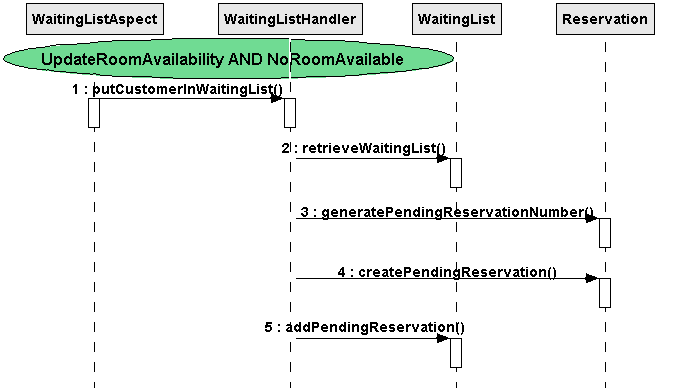
\includegraphics[scale=0.5]{img/case_study_behavioral_waiting_list.png}
	\caption{Advice behavior of the crosscutting concern to handle a waiting list.}\label{fig:case_study_behavioral_waiting_list}
  \end{figure}
  
   \begin{figure}
	\centering
	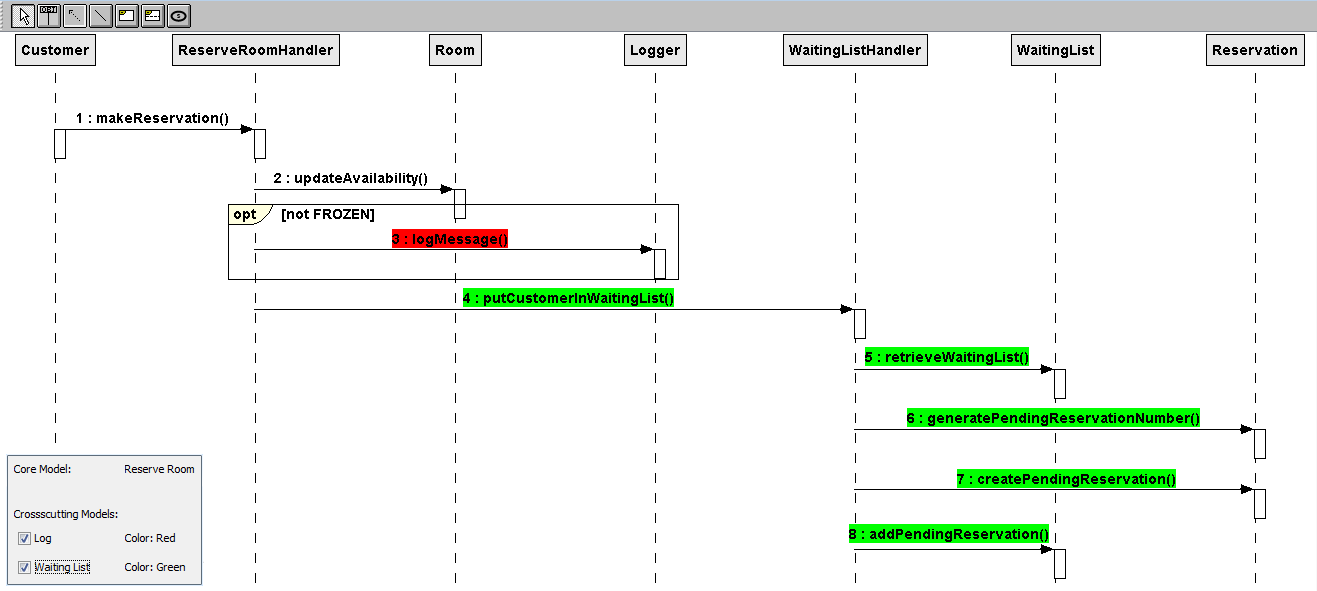
\includegraphics[scale=0.3]{img/case_study_compound_2.png}
	\caption{Case Study: Reserve
	Room composed with Log and Waiting List.}\label{fig:case_study_compound_2}
  \end{figure}
  
After the modeling of all the core and crosscutting concerns, the modeler may interchange the model views, selecting which concerns he wants to see
composed in the same diagram. The SEA/Aspect tool allows the selection of more than one model to be composed at the same time. Figure
\ref{fig:case_study_compound_2} shows a compound model, with the concerns of reserve room, log and waiting list composed together. The compound
diagram shows the model selector in it is right bottom, that allows changing the models that are being show. The messages of different concerns are
illustrated with different colors, as each concern has a color associated with it. This is useful to differentiate which messages comes from which
aspect in the compound model.
  
\section{Conclusion}

This work has proposed an approach to model aspect-oriented systems using UML, with a lightweight profile that allows to implement an aspect
visualizer in the SEA environment. The SEA/Aspect tool performs the composition between core and crosscutting models automatically, allowing the visualization of
the aspect dynamics in a system.

The main advantages of the proposed approach in relation to the others are: the representation of the important characteristics of the AOP, like the
capture of multiple join points with the representation of the aspect behavior; the definition of a profile within the UML standards, which can be
added in CASE tools that support importing profiles, and the composition and automatic visualization of the effect of the aspects in the core models
in the SEA environment, which eases the understanding and maintenance of aspect-oriented systems.

\bibliography{document}

\end{document}